\documentclass[twocolumn, twoside]{article}

\usepackage{graphicx}
\usepackage{amsmath}
\usepackage{mathtools}
\usepackage{amssymb }
\usepackage{algorithm}
\usepackage{algorithmicx}
\usepackage{algpseudocode}
\usepackage{comment}
\usepackage{ctex}
\usepackage{fontspec}
\usepackage{listings}
\usepackage{xcolor}
\usepackage{blindtext}
\usepackage[hmarginratio=1:1,top=32mm,columnsep=20pt]{geometry} % Document margins
\usepackage[hang, small,labelfont=bf,up,textfont=it,up]{caption} % Custom captions under/above floats in tables or figures
\usepackage{booktabs} % Horizontal rules in tables
\usepackage{fancyhdr} % Headers and footers
\pagestyle{fancy} % All pages have headers and footers
\fancyhead{} % Blank out the default header
\fancyfoot{} % Blank out the default footer

\newfontfamily{\lstsansserif}[Scale=.85]{Consolas}

\begin{comment}
\usepackage{titlesec} % Allows customization of titles
\renewcommand\thesection{\Roman{section}} % Roman numerals for the sections
\renewcommand\thesubsection{\roman{subsection}} % roman numerals for subsections
\titleformat{\section}[block]{\large\scshape\centering}{\thesection.}{1em}{} % Change the look of the section titles
\titleformat{\subsection}[block]{\large}{\thesubsection.}{1em}{} % Change the look of the section titles
\end{comment}

% 添加索引
\usepackage{titling} % Customizing the title section
\usepackage{hyperref} % For hyperlinks in the PDF

\usepackage{subfig}

%列表
\usepackage{enumerate}
\usepackage[shortlabels]{enumitem}

\lstset{
   %行号位置
   numbers=left,
   %行号和代码距离
   numbersep=3mm,
   %背景框
   frame=single,
   %背景框左侧和代码边距
   framexleftmargin=6mm,
   %代码整体和页面左侧边距
   xleftmargin=6mm,
   %自动换行
   breaklines=true,
   %背景色
   %backgroundcolor=\color[rgb]{1,1,0.76},
   %backgroundcolor=\color[RGB]{245,245,244},
   %样式
   keywordstyle=\bf\color{blue},
   %identifierstyle=\bf,
   %numberstyle=\color[RGB]{0,192,192},
   commentstyle=\color[RGB]{0,96,96},
   %stringstyle=\rmfamily\slshape\color[RGB]{128,0,0},
   %显示空格
   showstringspaces=false,
   breakatwhitespace=false,
   %字体大小
   basicstyle=\small\lstsansserif
}
%opening
\title{}
\author{}

\begin{document}

%\maketitle

%\begin{abstract}

%\end{abstract}

\section{使用示例}
\subsection{伪代码}

\begin{algorithm}
 \caption{pseudocode test}
 \label{pse:test}
 \scriptsize
 \begin{algorithmic}[1]
 \If {$left < right$}
    \State $middle \gets (left + right) / 2$
    \State $result \gets result +$ \Call{sort}{$Array, left, middle$}
    \State $result \gets result +$ \Call{sort}{$Array, middle, right$}
    \State $result \gets result +$ \Call{merg}{$Array,left,middle,right$}
    
 \EndIf
\end{algorithmic}

\end{algorithm}
使用: Algorithm \ref{pse:test}

\subsection{公式}
\begin{equation}\label{eq:v1}
\resizebox{.95\linewidth}{!} {$
\begin{array}{l}
\Delta V = \left\{\begin{array}{l}  \Delta H \\
\phantom{\hspace{4.8cm}} if \  a = b  \\  \\
 1 \\ 
\phantom{\hspace{3.8cm}} if \ \Delta H \geqslant \left\{\begin{array}{l}
1 \\ \Delta V
\end{array}\right. \\ \\
G  \\
\phantom{\hspace{3.8cm}} if \ G \geqslant \left\{\begin{array}{l}
\Delta H \\ \Delta V
\end{array}\right. \\ \\
\begin{array}{l}
\Delta V +  G  - \Delta H 
\end{array} \\
\phantom{\hspace{3.8cm}} if \ \Delta V \geqslant \left\{\begin{array}{l}
I-G\\ \Delta H
\end{array}\right.
\end{array}\right.
\\ \\
where \ i \in [1,m], \ j \in [1,n]
\end{array}
$}
\end{equation}

使用: Equation \eqref{eq:v1} 

\blindtext
\subsection{代码}

\begin{figure}[!htb]
\centering
\begin{lstlisting}[language={C}]
int64_t total_size = in_arg->total_size;
int bucket_num = in_arg->bucket_num;

\end{lstlisting}
\caption{A sample code}\label{fig:code}
\end{figure}

使用:Figure \ref{fig:code}

\subsection{图片}

\begin{figure}[!htb]
\centering
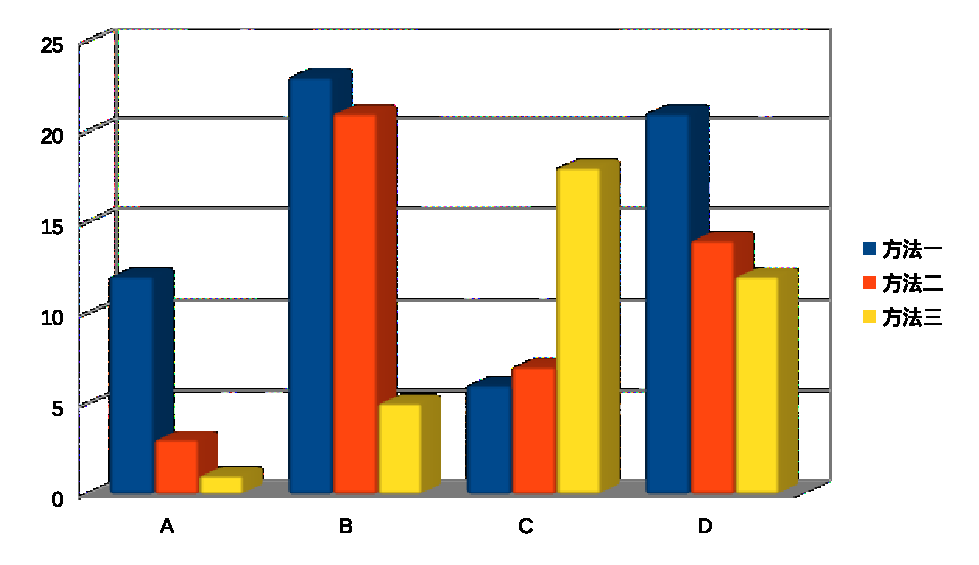
\includegraphics[width =\linewidth]{figure/simple.eps}
\caption{A simple figure}\label{fig:simple}
\end{figure}

使用:Figure \ref{fig:simple}    Figure \ref{fig:column}    Figure \ref{fig:column:a}    Figure \ref{fig:column:b}   


\begin{figure*}[!htb]
\centering
  \subfloat[figure a]{ 
    \label{fig:column:a} %% label for first subfigure 
      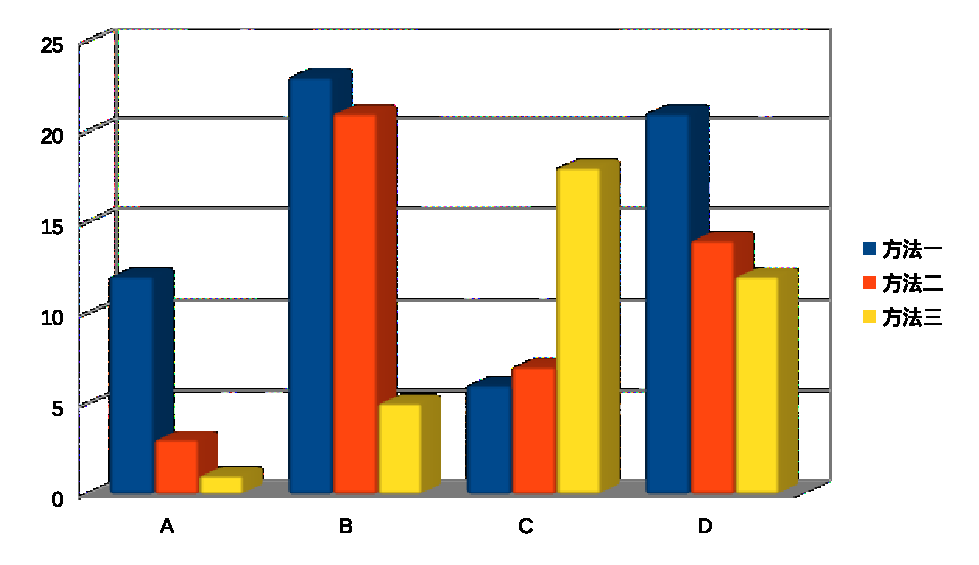
\includegraphics[width=0.5\linewidth]{figure/simple.eps} }
   \subfloat[figure b ]{ 
    \label{fig:column:b} %% label for first subfigure 
      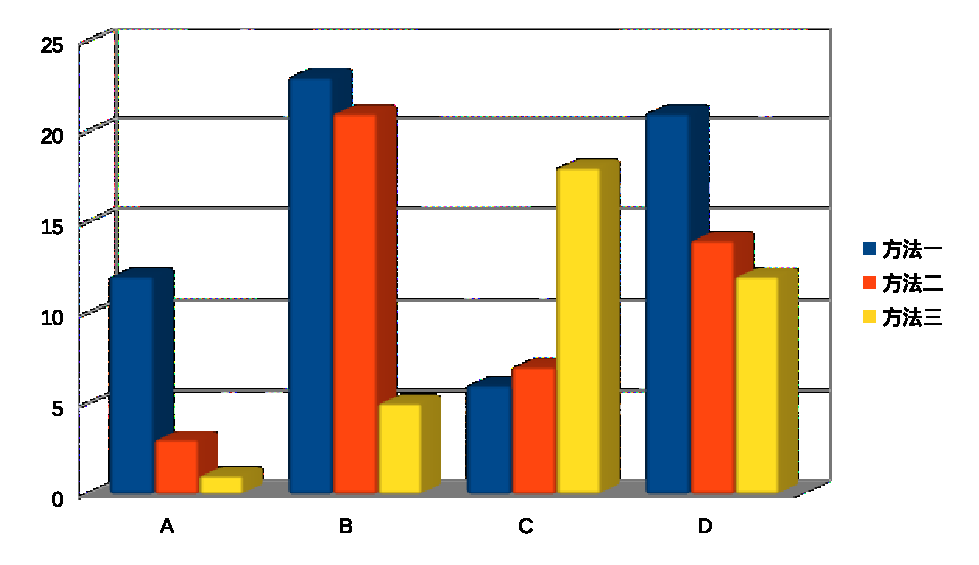
\includegraphics[width=0.5\linewidth]{figure/simple.eps} }
  \caption{A sample of two columns figure.} 
  \label{fig:column} %% label for entire figure

\end{figure*}
\blindtext

\subsection{列表}

\begin{enumerate}[1)]
\item This is item 1.
\item This is item 2.
\end{enumerate}

\begin{enumerate}[*]
\item This is item 1.
\item This is item 2.
\end{enumerate}

\subsection{表格}
% Please add the following required packages to your document preamble:
% \usepackage{booktabs}
% \usepackage{graphicx}
在线工具: \href{http://www.tablesgenerator.com/}{LaTeX Table Generator}. 

使用: Table \ref{tab:t1} Table \ref{tat:t2}
\begin{table}[!htb] 
\centering
\caption{Style 1}
\label{tab:t1}
\resizebox{\linewidth}{!}{%
\begin{tabular}{@{}lll@{}}
\toprule
\multicolumn{3}{c}{Item} \\ \midrule
Animal & Descprition & Price (\$) \\
Gnat & per gram each & 13.66 \\ \bottomrule
\end{tabular}%
}
\end{table}


\begin{table}[!htb]
\centering
\caption{Style 2}
\label{tat:t2}
\resizebox{\linewidth}{!}{%
\def\arraystretch{1.3} % 设置行高度
\begin{tabular}{|c|c|c|}
\hline
\multicolumn{3}{|c|}{Item} \\ \hline
Animal & Descprition & Price (\$) \\ \hline
Gnat & per gram each & 13.66 \\ \hline
\end{tabular}%
}
\end{table}
\blindtext
\end{document}
